\documentclass[11pt,journal]{article}
%\usepackage{hyperref}
%\usepackage[breaklinks]{hyperref}
\usepackage{breakurl}
\usepackage{url}
\usepackage{listings}
\usepackage{courier}
\usepackage{amsmath}
\usepackage{graphicx}
\graphicspath{ {/home/agata/Documents/coursework/SensorNetworks/Lab2/} }
%\ifCLASSOPTIONcompsoc
% IEEE Computer Society needs nocompress option
% requires cite.sty v4.0 or later (November 2003)
\usepackage[nocompress]{cite}

%\else
% normal IEEE
\usepackage{cite}
%\fi

\hyphenation{op-tical net-works semi-conduc-tor}
\addtolength{\oddsidemargin}{-.875in}
\addtolength{\evensidemargin}{-.875in} 
\addtolength{\textwidth}{1.75in}

\addtolength{\topmargin}{-.875in}
\addtolength{\textheight}{1.75in}

\begin{document}
	\title{Sensor Networks and Mobile Data Comminucation, Assignment 2}
	
	\author{UID: 1690550}% <-this % stops a space
		%\protect\\
		%\thanks{}}
	
	% The paper headers



	% IEEEtran.cls defaults to using nonbold math in the Abstract.
	% This preserves the distinction between vectors and scalars. However,
	% if the journal you are submitting to favors bold math in the abstract,
	% then you can use LaTeX's standard command \boldmath at the very start
	% of the abstract to achieve this. Many IEEE journals frown on math
	% in the abstract anyway. In particular, the Computer Society does
	% not want either math or citations to appear in the abstract.
	
	% Note that keywords are not normally used for peerreview papers.
	
	% make the title area
	\maketitle
	
	
	% To allow for easy dual compilation without having to reenter the
	% abstract/keywords data, the \IEEEcompsoctitleabstractindextext text will
	% not be used in maketitle, but will appear (i.e., to be "transported")
	% here as \IEEEdisplaynotcompsoctitleabstractindextext when compsoc mode
	% is not selected <OR> if conference mode is selected - because compsoc
	% conference papers position the abstract like regular (non-compsoc)
	% papers do!
	%\IEEEdisplaynotcompsoctitleabstractindextext
	% \IEEEdisplaynotcompsoctitleabstractindextext has no effect when using
	% compsoc under a non-conference mode.
	
	
	% For peer review papers, you can put extra information on the cover
	% page as needed:
	% \ifCLASSOPTIONpeerreview
	% \begin{center} \bfseries EDICS Category: 3-BBND \end{center}
	% \fi
	%
	% For peerreview papers, this IEEEtran command inserts a page break and
	% creates the second title. It will be ignored for other modes.
	%\IEEEpeerreviewmaketitle
	\section{Preparation and initial readings}
	Before we could attempt to compare the different models ran with different parameters, some initial readings had to be taken. Originally, the readings were taken over a very narrow range of distances between nodes and the transmission power. Namely, the power ranged from 0.1 to 0.12 dBm, and the distance ranged from 180 to 180.9 m. No packets were received during the original simulation.
	
	We decided to look at a much wider range for both of these parameters. First we note that 802.11b standard lists 20 dBm as the standard transmission power for WiFi, with -100 dBm being the minimal received signal power. Using the default parameters for the model, we took readings at transmission power ranging from -10 dBm to 3 dBm, in 0.5 dBm intervals, and at distance in the range 10 m to 200 m, in 5 m intervals. Figure 1 show the maximum transmission distance for each of the power values.
	
	\begin{figure}[h]
		\centering
		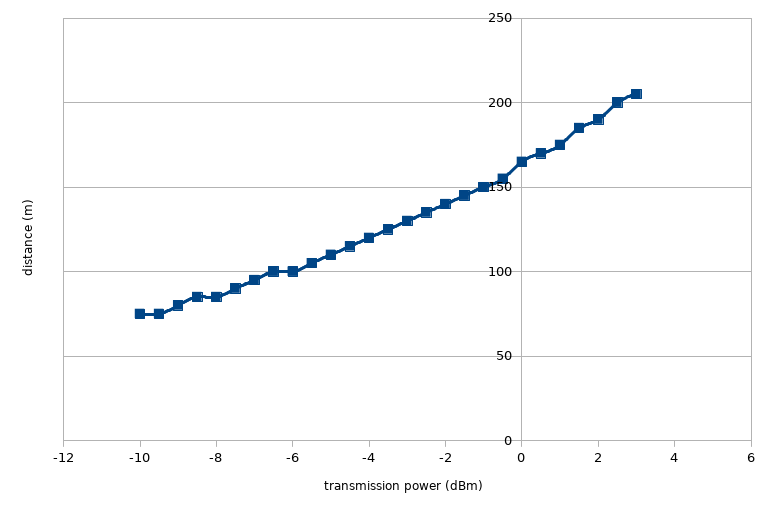
\includegraphics[scale=0.6]{graph_initial.png}
		\caption{Maximum transmission distance for the given transmission power.}
	\end{figure}

	These results will be considered the "normal" output, to which we can compare the outcomes of any modifications.
	
	
	
	\section{Log-distance propagation loss model (Methods 1)}
	The equation to calculate loss in the log-distance propagation model\footnote{\url{https://www.nsnam.org/docs/release/3.19/doxygen/classns3_1_1_log_distance_propagation_loss_model.html}} is:
	\[L = L_0 + 10nlog_{10}(\dfrac{d}{d_0})\] 
	with $L$ being the relative path loss, $L_0$ the path loss at reference distance $d_0$, n being the path loss distance exponent, and d the distance at which we're looking.
	
	The model has 3 attributes: path loss exponent, reference distance, and reference loss. Reference distance and loss come together, and we shall look at them first. This pair of attributes describes how much power we lose at the reference distance from the source. It is included in the model to avoid taking $log_{10}(0)$ which tends to $-\infty$. Therefore there is no point in attempting to get a reading at a shorter distance, as it will not be meaningful. 
	
	Effectively, these attributes describe how much to add to the loss, to account for skipping the reference distance in the calculations. It should not come as a surprise that increasing the reference loss, decreases transmission range. 
	
	We have measured the transmission distance, with reference loss ranging from 7 to 20 dB in 0.5 dB intervals, at transmission power -10 dBm. The outcome is shown in the graph below.
	
	\begin{figure}[h]
		\centering
		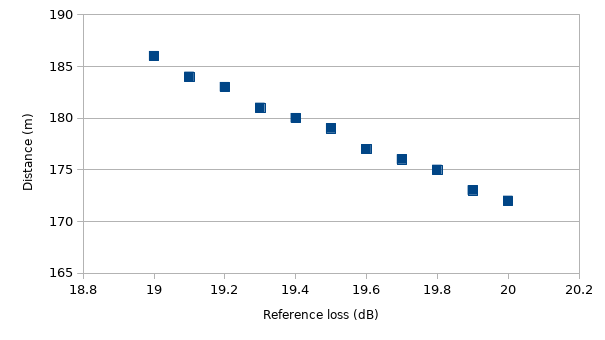
\includegraphics[scale=0.6]{graph_log_refloss.png}
		\caption{Maximum distance reached for a given reference loss.}
	\end{figure}
	
	It is not ideal to increase the reference distance, as it will limit the range at which we can take the readings. Attempting to find the loss at a distance less than the reference distance, will return the transmission power.

	The other parameter in the model is the exponent $n$. Recall the model equation:
		\[L = L_0 + 10nlog_{10}(\dfrac{d}{d_0})\] 
		\[ = L_o + 10log_{10}((\dfrac{d}{d_0})^n)\]
		
	Therefore, we can expect an exponential decrease in the maximum distance reached, as we increase the exponent. Our findings, summarised in the graph in Fig. 3 indeed demonstrate this trend. (Readings taken at transmission power -10 dBm.)
	
	
	\begin{figure}[h]
		\centering
		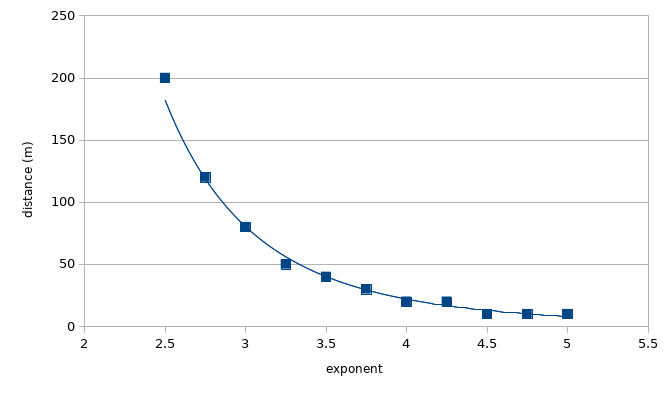
\includegraphics[scale=0.6]{graph_log_exponent.png}
		\caption{Maximum distance reached for a given exponent.}
	\end{figure}
	
	\section{Friis propagation loss model}
	This model has been first introduced by H. Friis in 1946\footnote{H. Friis, "A note on simple transmission formula" in \emph{Proc. IRE}, 1946}. 
	%\IEEEPARstart{}{} 
	

	
	% that's all folks
\end{document}

